\section{Introduction}

In many popular software projects, bug reports arrive with frequency and in bursts that can overwhelm even well-resourced and well-organized bug triage.
%
At the same time, a significant proportion of the arriving bug reports lack sufficient actionable information for bug triagers to reproduce the bug.
%
Researchers have observed this problem of bug report incompleteness (or inadequacy), e.g., reporting that over 60\% of bug reports lack any steps to reproduce and over 40\% lack any description of the expected behavior~\cite{chaparro17detecting}.
%
Missing information in bug reports was also a key concern in the first open letter to GitHub from the maintainers of open source projects~\cite{deargithub}, which was partially addressed via a bug report template mechanism.
%
While nowadays some of the software projects on GitHub rely on specific templates that bug reports must follow or publish bug reporting guidelines, there are many cases where templates are ignored and guidelines are poorly followed by reporters.
%
Bug triagers posing quick follow-up questions in order to elicit additional information from bug reporters is one method bug triagers use to augment the bug reports with necessary information.
%
However follow-up questions are only effective if they are posed quickly, before the user reporting the bug loses focus on the specifics.
%
In this paper, we examine how the posing such follow-up questions for inadequate bug reports can be performed automatically, designing and describing a system to reduce bug triage effort and improving overall bug report quality by automatically posing follow-up questions for inadequate bug reports.

\begin{figure}[ht]
\centering
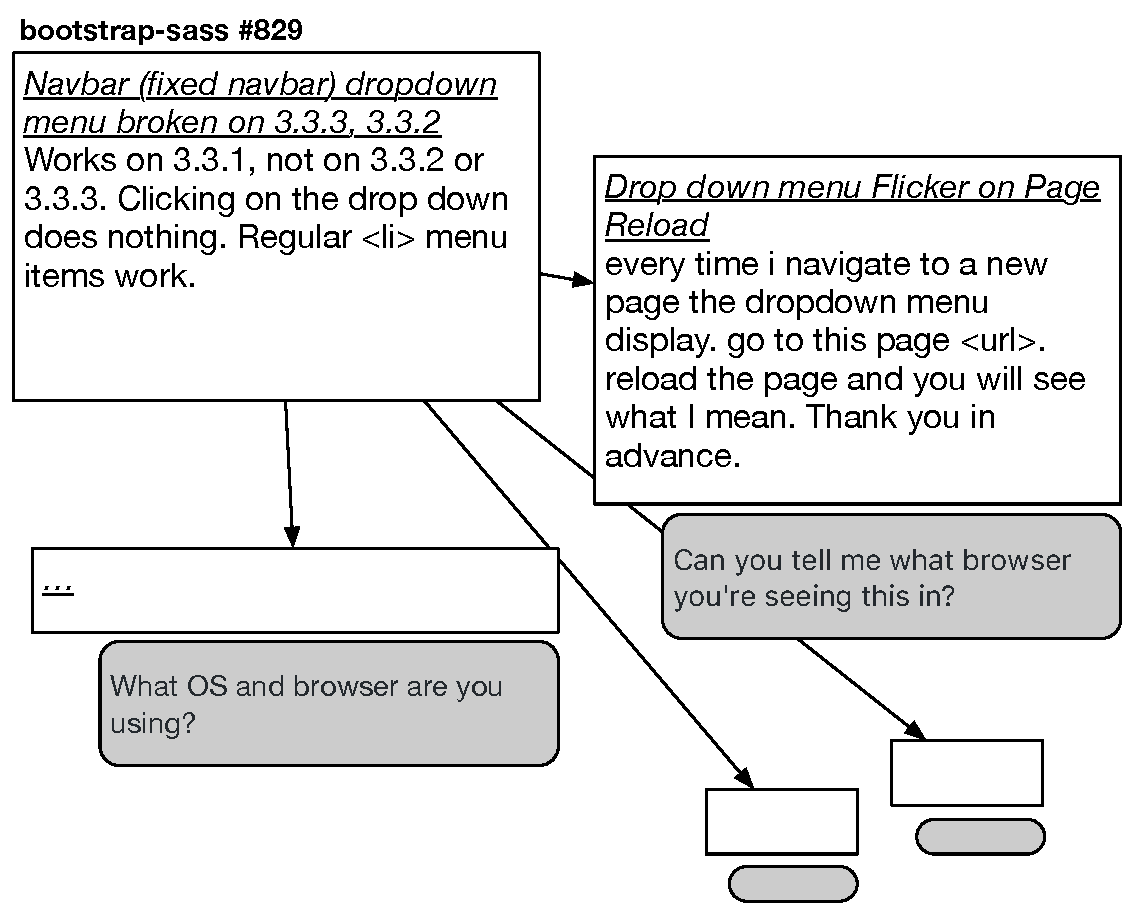
\includegraphics[width=0.99\linewidth]{figures/br_motivation.pdf}
\caption{The text for bug report (\#829) of the {\em bootstrap-sass} project is similar to other bug reports with already posed follow-up questions. Our system ranks this candidate set of follow-up questions based on the utility of the expected answer.}
\label{fig:repo_activity}
\end{figure}


%
We base our automatic follow-up question posing system on the following assumptions and ideas: 1) relevant follow-up question are common, not overly specific, and have already been posed in other prior bug reports in the current project or in others; 2) similar bug reports necessitate similar follow-up questions; and 3) the utility of the answer provided to a prior similar follow-up question is indicative of its value to the current bug report.
%
Based on this, our system performs an information retrieval task, locating the most relevant and useful follow-up question for a specific inadequate bug report, given a large corpus of previous bug reports, follow-up questions, and their answers.
%
For instance, consider the example shown in Figure 1, where the text of the bug report {\em boostrap-sass} \#829 is similar to several other bug reports on GitHub with existing follow-up questions.
%
In our system, choosing the right follow-up questions is a combination of this similarity between bug reports and the utility of the expected answer to the follow-up question.
%
A requirement for a system that locates such candidate follow-up questions and then ranks them in order of their perceived utility is a large-scale corpus.

To curate a corpus of prior bug reports, follow-up questions, and their answers we leverage GitHub, where we focus on popular repositories that have a high level of activity and therefore are likely to have numerous relevant follow-up questions, encoded as GitHub issue comments. We gather the answers to these follow-up questions that occur either as additional GitHub issue comments or as edits to the original bug report text. We base our estimate of the utility of an answer using the patterns to identify Observable Behavior (OB), Expected Behavior (EB) and Steps to Reproduce (S2R), published by Chaparro et al~\cite{chaparro17detecting}. We evaluate our prototype in two ways, based on the ability to predict an annotated held-out set of follow-up questions, and based on a developer survey that aims to gauge the usefulness of the follow-up questions we recommend. The results indicate that the technique is viable, with X MRR on the held-out set and Y\% of respondents indicating that the follow-up question is “bla bla bla”.

To summarize, the primary contributions of this paper are:
\begin{enumerate}
\item mechanism for automatically posing follow-up questions to aid with inadequate bug reports
\item metric to rank follow-up questions for a specific bug report based on their utility
\item process to curate a large corpus of existing follow-up question that can be used for recommendation
\end{enumerate}

Relative to the prior efforts by the software engineering research community towards improving the quality of bug reports, this paper is the first to propose follow-up questions. Automatically posing follow-up questions has been proposed in several other domains, e.g.,  for improving the quality of Web forum posts~\cite{rao-daume-iii-2018-learning}, product reviews in online retail, and improving query quality in Web search.

% More specifically, the contributions of this paper are:
%
% \begin{itemize}
% \item x
% \item y
% \item z
% \end{itemize}
